\section{Background}

\todo[inline]{Section introduction}

\subsection{Control Flow}

EBA provides a representation of the control flow of the input source files which is utilized in order to detect bugs. EBA generates a tree structure of the input, modeling statements as so-called \texttt{step}s. A path in this tree structure models a possible execution path, with each \texttt{step} in a path containing information about the modelled statements. The tree structure consists of $t$ nodes, which can be formalized as follows.

\begin{equation*} 
    \begin{aligned}
        t =\;& \mathit{Nil} \\
        & \mathit{Assume} (cond, bool, t) \\
        & \mathit{Seq} (step, t) \\
        & \mathit{If} (t, t) \\
    \end{aligned}
\end{equation*}

\noindent A few things are of note here; $Nil$ indicates the end of a path in the tree structure. $Assume$ is effectively ignored in my work, and is merely used in order to continue the exploration of the tree structure. $If$ indicates a branch in the input source file and models possible branches in if-statements. $Seq$ is the most interesting of $t$, since this type consists of the aforementioned $step$, providing access to information about the effects of a statement. It is also worth noting that all types provide the next $t$ in the current branch, allowing recursively exploring the tree until a $Nil$ is reached. 

\newpar $step$s contain information about a statement in the input source file, such as the type of statement, location of the statement and the effects of  the statement. The latter of the three is relevant for my analysis, since we are interested in monitoring effects of statements using monitor automata. A step contains two internal sets, each modelling which effects EBA analyzes a step \textit{must} and \textit{may} have. Each set consists of the effect type $e$, formalized below. 

\newpar Effects which operate on memory regions are modelled as the $Mem$ type. $Mem$ provides information about the type of effect and on which region the effects happen. Monitor automata can of course monitor all $e$s, but given that we are interested in detecting ressource manipulation errors and these ressources are stored in memory, $Mem$ is what I will describe in greater detail. The type of effect is modelled as $mem\_kind$, as seen in the definition of $e$. These types can be formalized as follows.

\begin{equation*} 
    \begin{split}
        \begin{aligned}
            e =\;   & \mathit{Mem} (mem\_kind, region) \\
                    & \mathit{Noret} \\
                    & \mathit{IrqsOn} \\
                    & \mathit{IrqsOff} \\
                    & \mathit{BhsOn} \\
                    & \mathit{BhsOff} \\
                    & \mathit{Var} (\mathit{effectvar}) \\
                    & \mathit{Sleep} \\
        \end{aligned}
    \end{split}
    \quad\quad\quad\quad\quad\quad\quad
    \begin{split}
        \begin{aligned}
            mem\_kind =\;   & \mathit{Alloc} \\
                            & \mathit{Free} \\
                            & \mathit{Read} \\
                            & \mathit{Write} \\
                            & \mathit{Uninit} \\
                            & \mathit{Call} \\
                            & \mathit{Lock} \\
                            & \mathit{Unlock} \\
        \end{aligned}
    \end{split}
\end{equation*}

\newpar A control flow defining effects of statements can be defined as a finite state machine $(\sum, S, s_0, \delta, F)$ as follows where $\sum$ is the input alphabet, $S$ is a finite non-empty set of states, $s_0$ is an element of $S$ and initial state, $\delta$ is the state-transition function $\delta: S \times \sum \rightarrow S$ and $F$ is the possibly empty set of final states and a subset of $S$. 

\subsection{Monitor Automata}
Monitor automata are defined as the quintuple $(\sum, S, s_0, \delta, F)$ where $\sum$ is the input alphabet, $S$ is a finite non-empty set of states, $s_0$ is an element of $S$ and initial state, $\delta$ is the state-transition function $\delta: S \times \sum \rightarrow S$ and $F$ is the possibly empty set of final states and a subset of $S$.

\newpar Monitor automata operate on the set of possible effects of a statement in the Control-flow Graph, which are defined as $E = \{$\texttt{alloc}, \texttt{free}, \texttt{read}, \texttt{write}, \texttt{uninit}, \texttt{call}, \texttt{lock}, \texttt{unlock}$\}$ by Abal \cite{EffectiveBugFinding}. These have been defined previously as the internal type, $mem\_kind$, generated by EBA. 

\newpar Monitor automata in this thesis all operate on a subset of $E$ and have a non-empty set of final states, $F$, indicating that a possible bug is discovered.  

\subsubsection{Double-unlock monitor automata}

A double-unlock monitor automata is defined as the quintuple $(\sum, S, s_0, \delta, F)$ where: 

\begin{itemize}
    \item $\sum = \{\texttt{unlock}, \texttt{lock}\}$, a subset of $E$
    \item $S = \{ locked_\rho, unlocked_\rho, error_\rho \}$, bound to a region $\rho$
    \item $s_0 = unlocked_\rho$ 
    \item $\delta =$ the relation $\{(locked_\rho, \texttt{unlock}_\rho, unlocked_\rho), (locked_\rho, \texttt{lock}_\rho, locked_\rho), \\
        (unlocked_\rho, \texttt{lock}_\rho, locked_\rho), (unlocked_\rho, \texttt{unlock}_\rho, error_\rho)\}$ 
    \item $F = error_\rho$  
\end{itemize}

An illustration of this monitor automata can be seen in figure \ref{double-unlock-automata}. 

\begin{figure}[H]
    \centering
    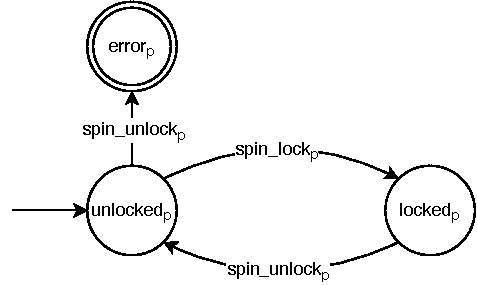
\includegraphics[width=0.5\textwidth]{background/figures/double-unlock}
    \caption{An illustration of a double-unlock monitor automata.}
    \label{double-unlock-automata}
\end{figure}
    
\subsubsection{Double-lock monitor automata}

A double-lock monitor automata is defined as the quintuple $(\sum, S, s_0, \delta, F)$ where: 

\begin{itemize}
    \item $\sum = \{\texttt{lock}, \texttt{unlock}\}$, a subset of $E$
    \item $S = \{ locked_\rho, unlocked_\rho, error_\rho \}$, bound to a region $\rho$
    \item $s_0 = unlocked_\rho$ 
    \item $\delta =$ the relation $\{(unlocked_\rho, \texttt{lock}_\rho, locked_\rho), (locked_\rho, \texttt{unlock}_\rho, unlocked_\rho), \\
    (locked_\rho, \texttt{lock}_\rho, error_\rho), (unlocked_\rho, \texttt{unlock}_\rho, unlocked_\rho)\}$ 
    \item $F = error_\rho$  
\end{itemize}

An illustration of this monitor automata can be seen in figure \ref{double-lock-automata}. 

\begin{figure}[H]
    \centering
    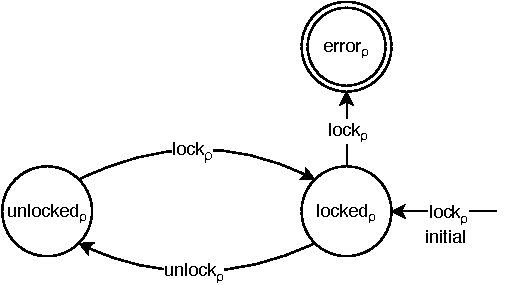
\includegraphics[width=0.5\textwidth]{background/figures/double-lock}
    \caption{An illustration of a double-lock monitor automata.}
    \label{double-lock-automata}
\end{figure}

\subsubsection{Double-free monitor automata}

A double-free monitor automata is defined as the quintuple $(\sum, S, s_0, \delta, F)$ where: 

\begin{itemize}
    \item $\sum = \{\texttt{free}, \texttt{alloc}\}$, a subset of $E$
    \item $S = \{ allocated_\rho, freed_\rho, error_\rho \}$, bound to a region $\rho$
    \item $s_0 = freed_\rho$ 
    \item $\delta =$ the relation $\{(freed_\rho, \texttt{alloc}_\rho, allocated_\rho), (allocated_\rho, \texttt{free}_\rho, freed_\rho), \\
    (freed_\rho, \texttt{free}_\rho, error_\rho), (allocated_\rho, \texttt{alloc}_\rho, allocated_\rho)\}$ 
    \item $F = error_\rho$  
\end{itemize}

An illustration of this monitor automata can be seen in figure \ref{double-free-automata}. 

\begin{figure}[H]
    \centering
    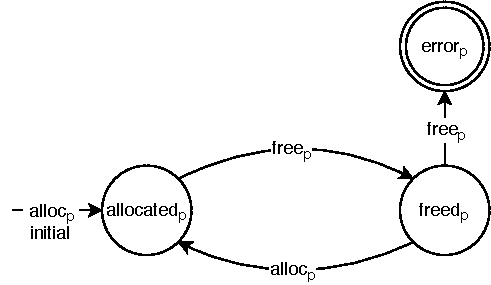
\includegraphics[width=0.5\textwidth]{background/figures/double-free}
    \caption{An illustration of a double-free monitor automata.}
    \label{double-free-automata}
\end{figure}

\subsubsection{Use-before-init monitor automata}

A use-before-init monitor automata is defined as the quintuple $(\sum, S, s_0, \delta, F)$ where: 

\begin{itemize}
    \item $\sum = \{\texttt{read}, \texttt{init}\}$, a subset of $E$
    \item $S = \{ unread_\rho, initialized_\rho, error_\rho \}$, bound to a region $\rho$
    \item $s_0 = unused_\rho$ 
    \item $\delta =$ the relation $\{(unread_\rho, \texttt{init}_\rho, initialized_\rho), (initialized_\rho, \texttt{uninit}_\rho, unread_\rho), \\
    (unread_\rho, \texttt{read}_\rho, error_\rho), (initialized_\rho, \texttt{init}_\rho, initialized_\rho)\}$ 
    \item $F = error_\rho$  
\end{itemize}

An illustration of this monitor automata can be seen in figure \ref{use-before-automata}. 

\begin{figure}[H]
    \centering
    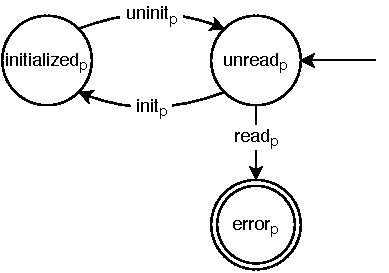
\includegraphics[width=0.5\textwidth]{background/figures/use-before}
    \caption{An illustration of a use-before-init monitor automata.}
    \label{use-before-automata}
\end{figure}